\documentclass[11pt,a4paper]{article}

\usepackage[margin=2.4cm,top=2.6cm,bottom=2.6cm]{geometry}
\usepackage{fontspec}
\usepackage{booktabs}
\usepackage{graphicx}
\usepackage{xcolor}
\usepackage{titlesec}
\usepackage{caption}
\usepackage{longtable}
\usepackage{array}
\usepackage{enumitem}
\usepackage{amsmath}
\usepackage[hidelinks]{hyperref}
\usepackage{fancyhdr}

\setmainfont{Palatino}
\setsansfont{Helvetica Neue}[Scale=MatchLowercase]
\setmonofont{Menlo}[Scale=0.85]

\definecolor{ink}{HTML}{0B0B0B}
\definecolor{ink2}{HTML}{52514E}
\definecolor{muted}{HTML}{898781}
\definecolor{rule}{HTML}{C3C2B7}
\definecolor{accent}{HTML}{2A78D6}
\definecolor{warn}{HTML}{D03B3B}

\titleformat{\section}{\sffamily\Large\bfseries\color{ink}}{\thesection}{0.7em}{}
\titleformat{\subsection}{\sffamily\large\bfseries\color{ink}}{\thesubsection}{0.6em}{}
\titleformat{\subsubsection}{\sffamily\normalsize\bfseries\color{ink2}}{\thesubsubsection}{0.6em}{}
\titlespacing*{\section}{0pt}{2.2ex plus 1ex minus .2ex}{1.1ex plus .2ex}

\captionsetup{font={sf,small,color=ink2},labelfont={bf},skip=6pt}
\setlength{\parskip}{0.62em}
\setlength{\parindent}{0pt}
\renewcommand{\arraystretch}{1.15}

\pagestyle{fancy}
\fancyhf{}
\renewcommand{\headrulewidth}{0.4pt}
\fancyhead[L]{\sffamily\footnotesize\color{muted}Buffett Quality--Value Ranking}
\fancyhead[R]{\sffamily\footnotesize\color{muted}\thepage}

\newcommand{\keyfinding}[1]{%
  \par\vspace{0.4em}%
  \noindent\colorbox{ink!4}{\parbox{\dimexpr\linewidth-2\fboxsep}{\vspace{0.3em}#1\vspace{0.3em}}}%
  \par\vspace{0.4em}}

\begin{document}

\thispagestyle{empty}
\begin{center}
\vspace*{1.2cm}
{\sffamily\Huge\bfseries The Buffett Quality--Value Ranking}\\[0.5em]
{\sffamily\Large\color{ink2} Method, Implementation, and a Point-in-Time Backtest}\\[1.4em]
{\sffamily\large\color{muted} United States listed equities, 2013--2025}\\[0.8em]
{\sffamily\normalsize\color{muted} Investa research note \quad\textbullet\quad 28 July 2026}
\end{center}

\vspace{1.2cm}

\hrule height 0.4pt
\vspace{0.9em}

\section*{\sffamily Executive summary}
\addcontentsline{toc}{section}{Executive summary}

This note documents a systematic implementation of Warren Buffett's investment
criteria as a cross-sectional ranking of the entire US listed universe, and
reports a point-in-time backtest of the resulting strategy over thirteen years.

\begin{enumerate}[leftmargin=1.4em,itemsep=0.35em]
  \item \textbf{The production blend does not beat the market.} Holding the top
  20 names by the shipped 60/40 quality--value composite, equally weighted and
  rebalanced each January, returned \textbf{13.6\%} a year over 2013--2025
  against \textbf{14.7\%} for the S\&P 500 total return index.

  \item \textbf{Shifting the blend to 80\% quality lifts it to 16.9\% a year},
  ahead of the S\&P 500 by 2.2 points with a smaller maximum drawdown
  ($-23.9\%$ against $-27.5\%$). This is the single change supported by the
  evidence, and it is supported by a monotone gradient present in the training
  window, the held-out window and the full sample alike.

  \item \textbf{Almost everything else that was tested was noise.} A sweep of
  900 configurations --- concentration, market-capitalisation floors, momentum
  overlays, two-stage screens --- produced a set of training-window winners
  whose median held-out return (12.0\%) was \emph{below} that of the grid as a
  whole (12.4\%). Tuning made things worse out of sample.

  \item \textbf{No configuration beat the NASDAQ-100} (19.7\% a year). The
  screen never held the mega-cap technology names that drove that index: across
  2020--2025 a Magnificent Seven stock entered the top 20 in one year out of
  six.

  \item \textbf{The results are flattered by survivorship bias} and cover
  thirteen years rather than twenty, because SEC XBRL fundamentals do not
  reach further back. Both limits are quantified in \S6.
\end{enumerate}

\vspace{0.6em}
\hrule height 0.4pt

\clearpage
{\sffamily\large\bfseries Contents}\vspace{-1.6em}
\renewcommand{\contentsname}{}
\tableofcontents

\clearpage

\section{The Buffett method, and what it demands of a screen}

Buffett's public writing is remarkably consistent about what he is looking for,
and remarkably unlike what most quantitative value screens actually measure. A
faithful implementation has to take five ideas seriously.

\subsection{Quality first, price second}

The ordering is not a stylistic preference; it is the whole argument. In the
1989 letter to shareholders Buffett described the lesson of his own worst
purchases: ``It's far better to buy a wonderful company at a fair price than a
fair company at a wonderful price.'' A screen that ranks on discount-to-value
inverts this. It will reliably put at the top the companies the market expects
to shrink, because a business in permanent decline looks cheap against any
model that assumes it will not decline.

This has a concrete architectural consequence, described in \S3.4: quality
tests run as \emph{gates} before any price is considered, and a company that
fails one is removed from the ranking entirely rather than scored badly and
buried.

\subsection{Owner earnings, not accounting profit}

Buffett's 1986 appendix defines owner earnings as reported earnings plus
depreciation and amortisation, less the capital expenditure required to
maintain competitive position. The final term is the difficulty: no filer
discloses maintenance capital expenditure separately from growth capital
expenditure. The implementation substitutes total capital expenditure:
\[
\text{owner earnings} = \text{operating cash flow} - \text{capital expenditure}
\]
which understates the earnings of a company investing heavily in growth. That
is a deliberate direction to err in --- a quality screen should be conservative
about companies whose cash generation depends on assumptions.

\subsection{Durability, not the latest year}

A 30\% return on equity in one year is noise. Fifteen per cent in each of
twelve years is evidence of something structural. Consequently almost nothing
in the metric set is measured on the most recent year: profitability,
predictability and growth are medians, dispersions and long-window compound
growth rates computed over a ten-year window. The exception is genuine
balance-sheet \emph{state} --- what the company owes today --- which is read
from the latest period, because that is what it is.

This requirement is also what makes the data problem hard, and it is the
binding constraint on how far back the backtest can reach (\S6.2).

\subsection{Circle of competence, expressed as sector models}

Buffett's circle-of-competence discipline is usually read as advice to
individuals. For a screen it translates into something sharper: a valuation
model applied outside its domain produces a confident, meaningless number. A
discounted-cash-flow valuation of a bank is not a poor estimate; it is an
answer to the wrong question, because for a deposit-taking institution
liabilities are the raw material of the business rather than a financing
choice, and ``free cash flow'' is not a coherent quantity.

The implementation routes every company to one of four models on its SEC
Standard Industrial Classification code (\S3.5).

\subsection{Margin of safety}

Graham's principle, which Buffett calls the three most important words in
investing, is that the estimate of value must exceed the price by enough to
absorb the estimate being wrong. This is implemented not as a haircut to a
point estimate but as a rank on the \emph{25th percentile} of a Monte Carlo
distribution of intrinsic value (\S3.6), on the reasoning that the mean of a
valuation distribution is not a price anyone should pay.

\section{Design principles}

Eight principles govern the implementation. They are stated here because
several of them constrain the code in ways that are not obvious from the
outputs.

\begin{description}[leftmargin=2.6em,style=nextline,itemsep=0.3em]
  \item[P1 --- Gates before scoring.] Solvency and persistent-loss tests remove
  a company from the ranked list and report it separately with a reason, rather
  than contributing a poor score.
  \item[P2 --- Conservative estimates over central ones.] Value is ranked on a
  low percentile of the valuation distribution; dispersion is penalised
  separately.
  \item[P3 --- Reuse the existing engine.] Ratios come from the same
  \texttt{financial\_ratios} module the rest of the application uses, so the
  ranking and the stock-detail view can never disagree about a company's ROE.
  \item[P4 --- Durability over level.] Medians and dispersions over a ten-year
  window, not point values.
  \item[P5 --- Explainability.] Every score decomposes into pillars and
  metrics, and every exclusion carries a machine-readable reason.
  \item[P6 --- Compare like with like.] All percentiles are computed
  \emph{within} a valuation model. A bank's equity-to-assets ratio is
  meaningful against other banks and meaningless against software companies.
  \item[P7 --- Missing data must never look good.] Every metric returns
  ``unknown'' rather than a default; unknowns flow into a confidence factor that
  can only demote. A gate fires only on a known violation.
  \item[P8 --- Point-in-time honesty.] Facts are stored keyed by filing
  accession, so the originally reported number remains available after a
  restatement. This is what makes \S5 a backtest rather than a hindsight
  exercise.
\end{description}

\section{Implementation}

\subsection{Universe}

The investable universe is built from the NASDAQ Trader symbol directories
(\texttt{nasdaqlisted.txt} and \texttt{otherlisted.txt}), which together list
every symbol on every US exchange. Filtering removes exchange-traded funds,
warrants, rights, units, preferred series, depositary receipts and test issues
--- roughly 13,000 raw rows reduce to about 5,600 common-stock listings. Each
is matched to an SEC Central Index Key so fundamentals can be retrieved.
Multiple share classes of one filer (BRK-A/BRK-B, GOOG/GOOGL) collapse to a
single company, since they share one set of financial statements.

\subsection{Fundamentals: SEC EDGAR XBRL}

The data source is the SEC's XBRL company-facts archive rather than a
commercial vendor, for a specific reason: vendor feeds available here return
four to five annual periods per company, and \S1.3 requires ten. EDGAR carries
roughly seventeen annual periods per filer at no cost.

Three implementation details matter for correctness:

\begin{itemize}[leftmargin=1.4em,itemsep=0.25em]
  \item \textbf{Only annual facts from annual reports} are retained.
  Quarterlies would let a company's fiscal calendar leak into cross-sectional
  comparisons. A ``duration'' fact counts as annual if it spans 300 to 400
  days, which accommodates the 52- and 53-week retail calendars.
  \item \textbf{Concepts resolve through fallback chains, period by period.}
  XBRL tag usage varies by company, by year and above all by industry. Apple's
  revenue arrives under \texttt{Revenues} for older years and
  \texttt{RevenueFromContractWithCustomer\dots} for newer ones; resolving per
  period rather than per company recovers one continuous series across the
  accounting-standard change.
  \item \textbf{Every (CIK, tag, period, accession) is its own row.} A
  restatement never overwrites the originally filed value. The resolver
  defaults to the most recent filing, but the originals remain --- which is
  precisely the mechanism \S5.1 depends on.
\end{itemize}

\subsection{Quality: five pillars}

Each metric is converted to a percentile within its valuation model, winsorised
at the 1st and 99th centiles so that a single absurd outlier --- a 10,000\%
return on equity computed from a near-zero equity base --- cannot compress every
other company into a narrow band. A pillar score is the mean of whichever of
its metrics resolved; the quality score is the weighted mean of the pillars,
renormalised over those present.

\begin{table}[h]
\centering
\sffamily\small
\begin{tabular}{@{}llp{7.4cm}@{}}
\toprule
\textbf{Pillar} & \textbf{Weight} & \textbf{Metrics (generic model)}\\
\midrule
Returns on capital & 30\% & Median ROE, median ROIC, median ROA, median gross margin, share of years with ROE above 15\%\\
Financial strength & 20\% & Debt-to-equity, interest coverage, current ratio, net debt to owner earnings\\
Predictability & 20\% & Dispersion of ROE, of revenue growth, of FCF margin; count of negative owner-earnings years\\
Growth & 15\% & Revenue CAGR, owner-earnings CAGR, book-value-per-share CAGR\\
Capital allocation & 15\% & Share-count CAGR (falling is good), incremental return on incremental capital\\
\bottomrule
\end{tabular}
\caption{Quality pillars and weights. Returns on capital carries the most
weight because a durable high return on capital \emph{is} the moat; growth
carries the least because growth without returns destroys value.}
\end{table}

Two metrics deserve comment. \textbf{Return on invested capital} nets cash off
the capital base, because a large idle balance would otherwise depress the
measured return on the operating business the moat question is actually about.
\textbf{Incremental return on incremental capital} --- the change in pre-tax
earnings divided by the change in equity across the window --- is the sharpest
available test of whether management creates value with retained earnings. It
is preferred to Buffett's own ``one dollar retained produces one dollar of
market value'' formulation because it requires no price history and therefore
cannot be contaminated by look-ahead bias.

\subsection{Gates}

Gates encode P1 and P7 together: a company is excluded for something its
filings \emph{show}, never for something they omit. Every test is written so
that a missing value cannot trigger it.

\begin{table}[h]
\centering
\sffamily\small
\begin{tabular}{@{}llp{6.6cm}@{}}
\toprule
\textbf{Gate} & \textbf{Threshold} & \textbf{Applies to}\\
\midrule
Insufficient history & $<8$ annual periods & all (relaxed to 5 in the backtest, \S6.3)\\
Interest not covered & coverage $<2.0$ & non-financials that report debt\\
Debt not serviceable & net debt / owner earnings $>6.0$ & non-financials\\
Persistent cash burn & $>2$ years of negative owner earnings & non-financials\\
Unprofitable & median ROE $<0$ & all except REITs\\
Undercapitalised & equity/assets $<4\%$ & banks, insurers\\
Persistent losses & $>2$ loss years & banks, insurers\\
Excessive leverage & debt/FFO $>15$ & REITs\\
\bottomrule
\end{tabular}
\caption{Quality gates. Roughly four fifths of the listed universe fails at
least one.}
\end{table}

The most instructive gate is the one that was \emph{removed}. Debt-to-equity
above 2.0 was the obvious solvency test and it was wrong: sustained buybacks
shrink book equity, so the ratio explodes for precisely the highest-quality
compounders. At that threshold it excluded 253 companies on that basis alone,
among them Apple --- which carried a debt-to-equity ratio of 3.9 alongside
\$99bn of annual owner earnings against \$55bn of net debt --- as well as ADP,
Amgen and American Express. Book equity is an accounting residual; the question
that matters is whether the business generates enough cash to retire what it
owes. Debt-to-equity survives as a \emph{scoring} input inside the financial
strength pillar, where a poor reading costs percentile points rather than
removing a company from consideration.

\subsection{Sector models}

\begin{table}[h]
\centering
\sffamily\small
\begin{tabular}{@{}lp{4.1cm}p{6.2cm}@{}}
\toprule
\textbf{Model} & \textbf{SIC range} & \textbf{Basis of measurement}\\
\midrule
Bank & 6020--6036, 6060--6062, 6080--6082, 6110--6120 & Residual income; equity/assets, net interest margin, provisioning, efficiency ratio\\
Insurer & 6311--6411 & Residual income, without lending metrics\\
REIT & 6798 & Funds from operations (NAREIT definition)\\
Generic & everything else & Free cash flow and the standard pillars\\
\bottomrule
\end{tabular}
\caption{Valuation model routing.}
\end{table}

SIC is used in preference to a vendor sector string because the distinctions
that matter here are exactly the ones vendor classifications blur. A
``Financial Services'' bucket mixes deposit-taking banks, which require a
residual-income model, with asset managers and exchanges, which have ordinary
free-cash-flow economics. Asset managers and brokers (SIC 6199, 6211) are
therefore deliberately \emph{not} treated as financials here.

Insurers were separated from banks after measurement showed that 29\% of
everything routed to the bank model had no deposits, no loan book and no net
interest income. Scoring those companies on lending metrics would have demoted
every one of them for lacking data they will never report --- a data gap
masquerading as poor quality, which is exactly what P7 exists to prevent.

For REITs, funds from operations replaces net income
($\text{FFO} = \text{net income} + \text{real-estate depreciation} - \text{gains
on property sales}$) because GAAP depreciation is charged on assets that in
practice hold or gain value. Share-count growth carries unusual weight in the
REIT model: REITs fund themselves by issuing equity, and growing FFO while
growing the share count faster is not growth.

\subsection{Value}

The value score blends a discounted-cash-flow margin of safety with classic
multiples, all ranked as percentiles within the valuation model.

\begin{table}[h]
\centering
\sffamily\small
\begin{tabular}{@{}lll@{}}
\toprule
\textbf{Component} & \textbf{Weight} & \textbf{Direction}\\
\midrule
Margin of safety (P25 of Monte Carlo) & 35\% & higher is better\\
Earnings yield & 20\% & higher is better\\
Free-cash-flow yield & 20\% & higher is better\\
EV/EBIT & 10\% & lower is better\\
Price/book & 10\% & lower is better\\
Price/sales & 5\% & lower is better\\
\bottomrule
\end{tabular}
\caption{Value components. The multiples carry more weight in aggregate than
the discounted cash flow because they rest on reported figures rather than on a
projected growth rate.}
\end{table}

Two refinements implement P2. First, the intrinsic value taken forward is the
25th percentile of the Monte Carlo distribution rather than the point estimate.
Second, a \emph{dispersion penalty} shrinks the margin of safety in proportion
to the width of that distribution, computed as $(P_{90}-P_{10})/P_{50}$: a
distribution twice as wide as its own midpoint has its margin roughly halved.
This is what stops a speculative business with a huge but meaningless apparent
discount from topping the value ranking. Where the discounted-cash-flow and
Graham models disagree by more than a factor of two, the lower of the two is
taken rather than the average, on the view that such disagreement is itself
evidence that neither should be trusted at face value.

Negative multiples are treated as missing rather than as cheap. A loss-making
company has no meaningful price-to-earnings ratio and a company with negative
book value has no meaningful price-to-book ratio; ranking them as ``cheapest''
would be an arithmetic accident.

\subsection{The composite}

\[
\text{score} = \bigl(w_Q \cdot \text{quality} + (1-w_Q) \cdot \text{value}\bigr)
\times \text{confidence}
\]

with $w_Q = 0.60$ as shipped. The confidence factor maps data coverage --- the
fraction of the model's headline metrics that resolved --- onto the interval
$[0.5, 1.0]$. It is capped at 1.0 so that it can only ever demote: full
coverage earns no bonus, it is merely the absence of a penalty. The floor
of 0.5 stops a thinly reported company from collapsing to zero and disappearing
silently instead of ranking low and visibly.

Where no value score is available the composite is quality alone, so the
ranking degrades gracefully when market data is missing rather than failing.

\section{Backtest methodology}

\subsection{Point-in-time fundamentals}

Every fact in the store carries the date it was filed. The backtest opens an
as-of context that restricts all reads to facts filed on or before the
rebalance date, so the January 2015 ranking sees only what had actually been
filed by 31 December 2014 --- the originally reported numbers rather than
subsequent restatements, and no fiscal year that had not yet been reported.

The mechanism was verified directly: in the 2015 ranking the latest fiscal
period visible for any company ends 1 November 2014. Apple's median return on
equity as of that date reads 29.6\%, against 119\% on today's data --- the
difference being a decade of buybacks shrinking the equity base. A backtest
using current data would have ranked the 2015 universe on a number that did not
exist in 2015.

\subsection{Prices in the money of the day}

Yahoo's closing prices are retroactively adjusted for splits. Multiplying such
a price by the share count a company reported at the time understates its
market capitalisation by the cumulative split factor --- fourfold for Apple,
fortyfold for NVIDIA. The backtest therefore reconstructs the price actually
quoted by multiplying the adjusted close by the product of all splits occurring
after that date.

Verified against known closes: Apple on 31 December 2014 reconstructs to
\$110.38 against an actual close of \$110.38; NVIDIA to \$20.05 against \$20.03;
Simon Property Group to \$182.11 against \$182.03. Share counts come from the
latest EDGAR filing available at the as-of date, and as-reported earnings per
share are used unmodified, so price, shares and per-share figures are all
expressed on the same basis. Returns are measured separately from the
dividend-and-split-adjusted series, so they are total returns.

\subsection{Portfolio construction}

At the first rebalance of each year the top $N$ names by composite score are
bought in equal weight and held for the calendar year, with weights left to
drift. A position whose price series ends mid-year --- delisting or acquisition
--- is frozen at its last quote and carried as cash for the remainder of the
year. Companies without a quote on the rebalance date are dropped rather than
ranked on quality alone, since they could not have been bought.

\section{Results}

\subsection{The production blend}

\begin{figure}[h]
\centering
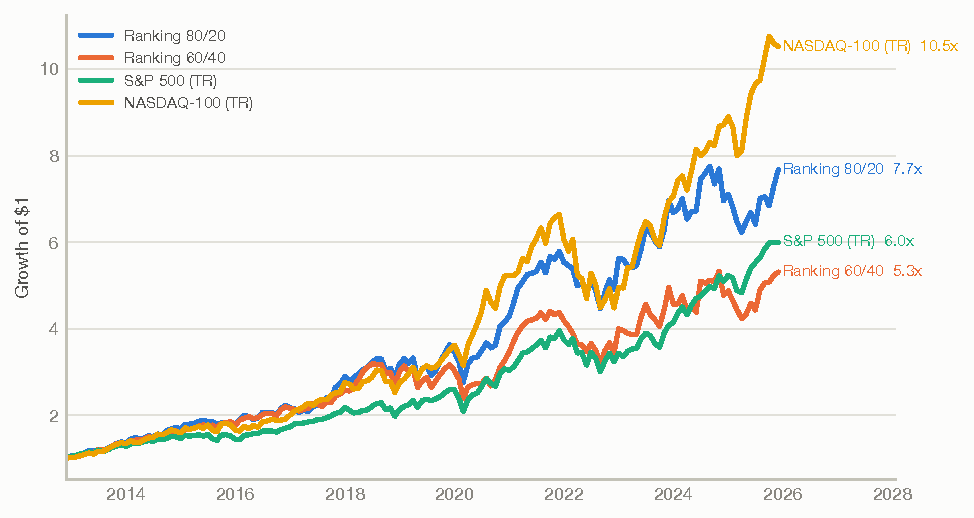
\includegraphics[width=\linewidth]{figures/fig1_growth.pdf}
\caption{Growth of one dollar, 2013--2025, monthly. The strategies are the top
20 names by composite score, equally weighted, rebalanced each January.
Benchmarks are total-return series, so dividends are included on both sides.}
\end{figure}

\begin{table}[h]
\centering
\sffamily\small
\begin{tabular}{@{}lrrrrr@{}}
\toprule
& \textbf{Total} & \textbf{CAGR} & \textbf{Volatility} & \textbf{Max drawdown} & \textbf{Return/vol}\\
\midrule
Ranking 80/20 (top 20) & 667.6\% & 16.9\% & 17.2\% & $-23.9\%$ & 0.98\\
Ranking 80/20, sector-capped & 613.6\% & 16.2\% & 17.1\% & $-24.3\%$ & 0.95\\
Ranking 60/40 (production) & 431.1\% & 13.6\% & 17.7\% & $-27.5\%$ & 0.77\\
S\&P 500 (total return) & 499.8\% & 14.7\% & 14.2\% & $-23.9\%$ & 1.04\\
NASDAQ-100 (total return) & 952.2\% & 19.7\% & 17.2\% & $-32.6\%$ & 1.15\\
\bottomrule
\end{tabular}
\caption{Summary statistics, 2013--2025. Volatility is annualised from monthly
returns; drawdown is measured on the monthly equity curve.}
\end{table}

\keyfinding{\textbf{The shipped configuration underperforms.} At 60/40 the
strategy returned 13.6\% a year against the S\&P 500's 14.7\%, with higher
volatility and a deeper drawdown. It beat the index in 7 of 13 years.}

The pattern of those wins is coherent rather than random. The screen won
2015, 2016, 2018 and the relative battle in 2022 --- the years when growth
stalled --- and lost heavily in 2019, 2020 and 2024, when mega-cap growth ran.
That is what a quality-and-value screen does in a growth decade.

\subsection{The parameter search, and its main negative result}

Nine hundred configurations were evaluated: quality weight from 0 to 1,
concentration from 5 to 50 names, market-capitalisation floors from zero to
\$10bn, and 12-1 month momentum both as a filter and as a blended score
component. Each was scored on a training window (2013--2019) and re-measured on
a held-out window (2020--2025) it had played no part in selecting.

\keyfinding{\textbf{The top 15 configurations by training-window return had a
median held-out return of 12.0\%, against 12.4\% for the grid as a whole.}
Selecting on the training window produced worse out-of-sample results than
choosing at random from the same grid.}

Individual configurations swung violently between the two windows: one that
returned 24.3\% in training delivered 4.3\% out of it. Momentum is the clearest
illustration: weighting it at 0.5 was
the \emph{worst} setting in training (12.4\% median) and the \emph{best} in the
held-out window (14.6\%). That is a regime effect, not an edge, and any
conclusion drawn from either window alone would have been wrong.

\subsection{The one change that survives}

\begin{figure}[h]
\centering
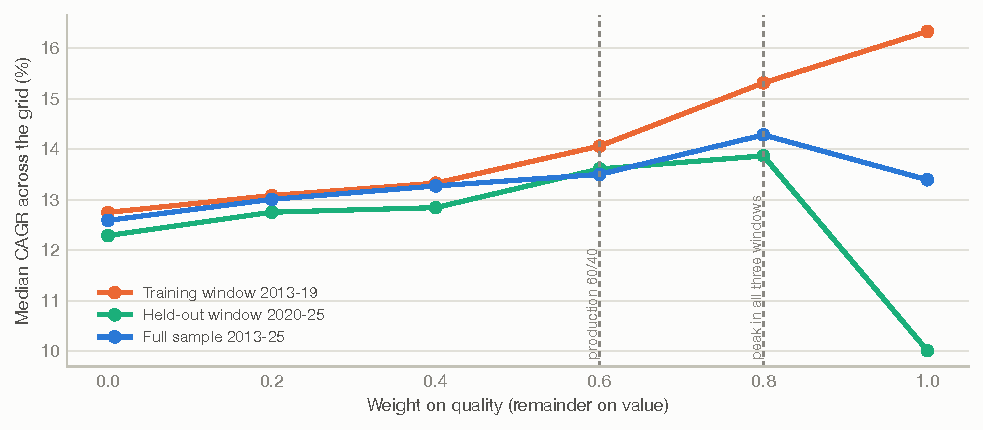
\includegraphics[width=\linewidth]{figures/fig3_quality_weight.pdf}
\caption{Median compound return across the entire grid, by weight on quality.
Each point is the median over every other setting --- concentration, market-cap
floor, momentum --- so it measures the effect of the weight alone rather than
of one favourable combination.}
\end{figure}

The gradient is monotone from 0 to 0.8 in all three windows, and only the
quality-only extreme (1.0) collapses out of sample, from a median of 13.9\% at
0.8 to 10.0\%. A single-parameter change supported by a consistent slope is far
weaker evidence of overfitting than the argmax of a noisy 900-cell grid, which
is why it is the only change recommended here.

\begin{figure}[h]
\centering
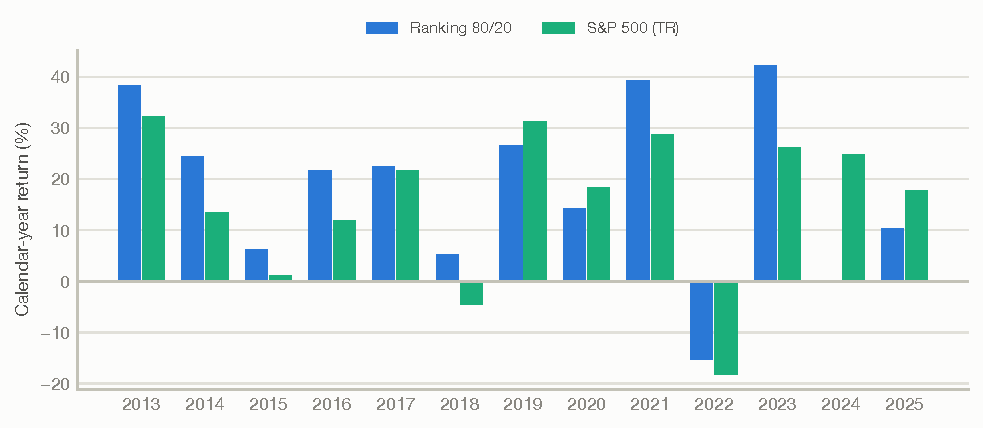
\includegraphics[width=\linewidth]{figures/fig2_annual.pdf}
\caption{Calendar-year returns, 80/20 ranking against the S\&P 500 total return
index. The strategy beat the index in nine of thirteen years, and the excess is
not concentrated in any single year.}
\end{figure}

At 80/20 the strategy returns 16.9\% a year, beating the S\&P 500 by 2.2 points
with a marginally smaller drawdown. It improves on the 60/40 blend in nine of
thirteen individual years. Concentration is a stable plateau from 10 to 20
names (top 10 returns 18.4\%); five names is fragile, returning 24.3\% in
training and 4.3\% in the held-out window.

\subsection{Industry concentration}

The ranking scores companies one at a time and has no representation of
correlation, so it will fill a fifth of the book with companies sharing a
single risk factor. In the current live ranking, four of the top twenty are
mortgage insurers (SIC 6351) and two more are homebuilders (SIC 1531): 30\% of
the portfolio on one macroeconomic exposure.

A cap on names per industry was implemented and tested.

\begin{table}[h]
\centering
\sffamily\small
\begin{tabular}{@{}lrrrrr@{}}
\toprule
\textbf{Rule (80/20, top 20)} & \textbf{CAGR} & \textbf{Return/vol} & \textbf{Max DD} & \textbf{Train} & \textbf{Held-out}\\
\midrule
No cap & 16.9\% & 0.98 & $-23.9\%$ & 20.0\% & 13.1\%\\
Max 3 per 2-digit SIC & 16.2\% & 0.95 & $-24.3\%$ & 19.1\% & 12.7\%\\
Max 3 per 3-digit SIC & 16.1\% & 0.92 & $-25.4\%$ & 19.8\% & 11.6\%\\
Max 2 per 3-digit SIC & 15.5\% & 0.89 & $-27.3\%$ & 18.6\% & 11.8\%\\
Max 1 per 3-digit SIC & 15.3\% & 0.85 & $-24.5\%$ & 18.7\% & 11.3\%\\
\bottomrule
\end{tabular}
\caption{The cost of capping industry concentration.}
\end{table}

\keyfinding{\textbf{Capping cost return and did not reduce drawdown.} Tighter
caps were monotonically worse on every measure --- the concentrated industries
happened to contain the better picks. The caveat cuts the other way: the sample
contains no housing crisis, which is precisely the event the cap insures
against. A backtest cannot price a tail that did not occur in it.}

Note also what a SIC cap cannot see. Mortgage insurance (6351) and homebuilding
(1531) are different industries carrying the same housing exposure, and no
classification-based cap will group them. Controlling that requires an explicit
factor bucket.

\subsection{The Magnificent Seven}

Across 2020--2025, a Magnificent Seven constituent entered the top 20 in one
year: 2023, when Meta ranked 7th and Alphabet 15th.

\begin{table}[h]
\centering
\sffamily\small
\begin{tabular}{@{}lrrrrrrr@{}}
\toprule
\textbf{Year} & \textbf{AAPL} & \textbf{MSFT} & \textbf{GOOG} & \textbf{AMZN} & \textbf{NVDA} & \textbf{META} & \textbf{TSLA}\\
\midrule
2020 & 261 & 119 & 310 & 731 & 374 & 148 & ---\\
2021 & 771 & 93 & 222 & 727 & 416 & 171 & ---\\
2022 & 586 & 78 & 189 & 564 & 337 & 58 & ---\\
2023 & 559 & 47 & \textbf{15} & 403 & 469 & \textbf{7} & ---\\
2024 & 634 & 89 & 228 & --- & 693 & 219 & ---\\
2025 & 965 & 79 & 223 & 985 & 34 & 108 & ---\\
\bottomrule
\end{tabular}
\caption{Rank under the 80/20 blend, out of roughly 1,100--1,250 ranked
companies. A dash means the company failed a quality gate that year. Tesla
failed one in every year of the sample.}
\end{table}

Their quality scores were strong throughout --- Microsoft 67--74, Alphabet
69--74, all around the top decile --- and their value scores were punishing:
NVIDIA scored 7 in 2021, 13 in 2023 and 4 in 2024. The value half of the
composite is what excluded them, which is visible in the weighting itself:
Microsoft ranked 336th under 60/40 in 2021 and 93rd under 80/20. The same
company, moved 240 places by the weight alone.

For scale, an equal-weight Magnificent Seven portfolio rebalanced annually
returned 43.1\% a year over 2020--2025, with 32\% volatility and a $-47\%$
drawdown. No quality-and-value screen was going to hold those names at those
multiples, and that single omission accounts for most of the gap to the
NASDAQ-100.

\section{Limitations}

\subsection{Survivorship bias}

The universe is constructed from current listing files, so companies delisted,
acquired or bankrupted between 2013 and 2026 were never candidates in any year.
This flatters the strategy, and it flatters it asymmetrically: the index
benchmarks are survivorship-free. Acquisitions typically complete at a premium
and bankruptcies at a total loss, and neither appears here. Every strategy
figure in \S5 should be read as an upper bound. Correcting it requires a
historical constituent database, which is not available from free sources.

\subsection{Thirteen years, not twenty}

XBRL filing became mandatory for large filers only in 2009, and a 10-K carries
two years of comparatives. The store therefore holds fundamentals for 32
companies in fiscal 2005 and 298 in fiscal 2007.

\begin{table}[h]
\centering
\sffamily\small
\begin{tabular}{@{}lrr@{}}
\toprule
\textbf{As of} & \textbf{Companies with any facts} & \textbf{With $\geq5$ annual periods}\\
\midrule
31 Dec 2011 & 865 & 26\\
31 Dec 2012 & 1,966 & 372\\
31 Dec 2013 & 2,042 & 862\\
31 Dec 2014 & 2,137 & 1,607\\
\bottomrule
\end{tabular}
\caption{Point-in-time data availability. 2013 is the earliest rebalance year
with a usable cross-section.}
\end{table}

\subsection{A relaxed history gate}

The production gate requires eight annual periods. At the end of 2014 that
threshold left 68 eligible companies out of roughly 4,000, which would have
made the early years meaningless. The backtest therefore requires five --- the
same floor the metrics module uses before it will compute a consistency measure
at all. Later years are effectively unaffected; the early years use a shorter
durability window than production does, which if anything understates the
quality signal.

\subsection{What the backtest does not model}

Transaction costs, bid-ask spreads, market impact and taxes are all excluded.
For an annually rebalanced 20-name book the turnover cost is small but not
zero. Some holdings are genuinely small companies where the assumption of
frictionless execution at a month-end close is optimistic --- and those are the
same names that survivorship bias most affects.

\section{Conclusion}

The ranking implements Buffett's criteria faithfully enough to be worth taking
seriously, and the exercise produced one durable result and one cautionary one.

The durable result is that \textbf{the quality half of the composite carries
the signal and the value half dilutes it}. Raising the quality weight from 0.60
to 0.80 moves the strategy from 1.1 points behind the S\&P 500 to 2.2 points
ahead, and the evidence for it is a monotone gradient present in every window
tested rather than the peak of a noisy search.

The cautionary result is that \textbf{almost everything else tested was
overfitting}. A grid large enough to contain an impressive answer will always
contain one; here the training-window winners were measurably worse than
average out of sample. Any future change to this ranking should be held to the
standard the quality weight met: a consistent effect across independent
windows, not a high score in one.

Two open questions follow. The screen has no mechanism to pay up for
durability --- a company can be the highest-quality business in the universe and
still be ranked out on price --- and whether that is a flaw or the entire point
is a judgement about investment philosophy that a backtest cannot settle.
Second, the value component deserves direct investigation: a 40\% weight on a
component that subtracts return is worth understanding before its scores are
trusted elsewhere in the application.

\appendix

\section{Reproducing these results}

\begin{table}[h]
\centering
\sffamily\footnotesize
\begin{tabular}{@{}lp{9.2cm}@{}}
\toprule
\textbf{File} & \textbf{Role}\\
\midrule
\texttt{src/edgar\_provider.py} & Fact store; the \texttt{as\_of()} context implementing P8\\
\texttt{src/buffett\_metrics.py} & Per-company metrics, all four sector models\\
\texttt{src/buffett\_rank.py} & Gates, pillar percentiles, the composite\\
\texttt{src/buffett\_value.py} & Margin of safety, dispersion penalty, multiples\\
\texttt{src/buffett\_pipeline.py} & End-to-end production run\\
\texttt{scripts/buffett\_backtest.py} & Point-in-time backtest\\
\texttt{scripts/buffett\_strategy\_search.py} & Parameter sweep and held-out evaluation\\
\texttt{scripts/buffett\_live\_picks.py} & Sized buy list from the latest run\\
\bottomrule
\end{tabular}
\end{table}

\begin{verbatim}
python scripts/buffett_backtest.py --start 2013 --end 2025 --top 20
python scripts/buffett_strategy_search.py --start 2013 --end 2025 --split 2019
python scripts/buffett_live_picks.py --capital 200000 --quality 0.8 \
    --max-per-sector 3 --sector-digits 2
\end{verbatim}

Per-year rankings are cached, so re-running with different parameters takes
seconds rather than minutes.

\section{Current portfolio}

Top 20 under the 80/20 blend with a cap of three names per 2-digit SIC group,
from the ranking run of 28 July 2026 (5,539 filers, 1,244 ranked), sized for
\$200,000 of capital.

\begin{table}[h]
\centering
\sffamily\footnotesize
\begin{tabular}{@{}llrrrr@{}}
\toprule
\textbf{Symbol} & \textbf{Industry} & \textbf{Price} & \textbf{Shares} & \textbf{Cost} & \textbf{Weight}\\
\midrule
MTG & Mortgage insurance & 30.00 & 333 & 9,990 & 5.00\%\\
RDN & Mortgage insurance & 39.33 & 254 & 9,990 & 4.99\%\\
ESNT & Mortgage insurance & 66.59 & 150 & 9,989 & 4.99\%\\
UNTY & Banks & 58.59 & 170 & 9,959 & 4.98\%\\
INVA & Pharma & 21.68 & 461 & 9,994 & 5.00\%\\
LULU & Apparel & 117.61 & 85 & 9,997 & 5.00\%\\
TSBK & Banks & 44.15 & 226 & 9,978 & 4.99\%\\
PKBK & Banks & 33.37 & 299 & 9,978 & 4.99\%\\
ADBE & Software & 237.72 & 42 & 9,984 & 4.99\%\\
GOOG & Software & 319.09 & 31 & 9,892 & 4.95\%\\
ACN & Software \& services & 154.20 & 64 & 9,869 & 4.93\%\\
PHM & Homebuilders & 129.29 & 77 & 9,956 & 4.98\%\\
G & Consulting & 32.35 & 309 & 9,996 & 5.00\%\\
XPEL & Fabricated metal & 43.66 & 229 & 9,999 & 5.00\%\\
MKTX & Brokers \& exchanges & 118.12 & 84 & 9,922 & 4.96\%\\
NVR & Homebuilders & 6,478.96 & 1 & 6,479 & 3.24\%\\
CPRT & Auto services & 29.49 & 339 & 9,997 & 5.00\%\\
ESRT & REITs & 5.62 & 1,779 & 9,998 & 5.00\%\\
AGM & Non-bank credit & 211.58 & 47 & 9,944 & 4.97\%\\
RMD & Instruments & 203.10 & 49 & 9,952 & 4.98\%\\
\midrule
\multicolumn{4}{@{}l}{\textbf{Invested}} & \textbf{195,865} & \textbf{97.9\%}\\
\bottomrule
\end{tabular}
\end{table}

Residual concentration after capping: 15.0\% mortgage insurance, 15.0\% banks,
14.9\% software and services, 8.2\% homebuilders. Mortgage insurance and
homebuilding together remain a 23\% exposure to US housing credit.

NVR at \$6,479 a share cannot fill a 5\% slot below roughly \$130,000 of
capital; fractional-share execution resolves this and puts the residual
\$4,135 of cash to work.

\vspace{1.2em}
\hrule height 0.4pt
\vspace{0.6em}
{\footnotesize\color{ink2}\sffamily This document reports the output of a
quantitative model on historical data. It is not investment advice, and past
results --- particularly backtested results carrying the biases described in
\S6 --- do not indicate future returns.}

\end{document}
